\setchapterimage{seaside}
\setchapterpreamble[u]{\margintoc}
\chapter{Template Chapter}
\labch{chaptertemplate}

%
% Key concepts and abilities
%==============================================================================
\begin{kaobox}[frametitle=In This Chapter]
you will learn
\begin{itemize}
	\item what is the first topic
	\item how to identify the second topic
        \item best practices for the third topic
\end{itemize}

you will be able to
\begin{itemize}
        \item perform the steps required to accomplish task one
        \item create a program that performs task two
\end{itemize}
\end{kaobox}

This introduction gives the reader any context necessary to understand the 
proceeding sections in this chapter.

The contents of the `In This Chapter' box should concrete. This should coorespond to
a `Chapter Review' section at the end of the chapter.

Illuminate any common obstacles for the reader. A few words of encouragement are also welcomed.

%
% Section: Heaps of Examples
%==============================================================================
\section{Heaps of Examples}
This section is fairly dense with examples. You can delete everything from here until
the end of the page.\sidenote[]{After you have saved this document as a new file.}

This section serves as an easy way to demonstrate\footnote{Like this footnote} multiple 
graphical elements\todo{Add a list of elements} that can be used in this book.

Keep chapters, sections, and sub sections capitalized.

%
% Subsection: Margin Stuff
%------------------------------------------------------------------------------
\subsection{Margin Stuff}
Generally, any text that would be written between parentheses would do well as
a margin note. Keep the flow going.

\marginnote{
	\begin{kaobox}[frametitle=Remember]
		a kaobox can be used in the margins for special reminders)
	\end{kaobox}
}

%
% Subsubsection: Sections in Depth
%
\subsubsection{Sections in Depth}
Sections within a chapter can be \Command{section}, \Command{subsection}, or
\Command{subsubsection}\marginnote{Notice that \Command{subsubsection} does not cause numbering.}.

%
% Subsection: Figures and Tables}
%------------------------------------------------------------------------------
\subsection{Figures and Tables}
\begin{lstlisting}[caption={
This Forth code does NOT generate \reftab{useless}
}]
: square  ( x -- x )
( Forth code that squares a number
    dup * ;
\end{lstlisting}

This is an example of a table contained withing the main column of text.

\begin{table}[ht]
\caption[A useless table]{A useless table.}
\labtab{useless}
\begin{tabular}{ c c c c }
    \toprule
    col1          & col2  & col3  & col4\\
    \midrule
    \multirow{3}{4em}{
    Multiple row} & 
        cell2 & cell3 & cell4\\ &
        cell5 & cell6 & cell7 \\ &
        cell8 & cell9 & cell10 \\
    \multirow{3}{4em}{
    Multiple row} & 
        cell2 & cell3 & cell4 \\ &
        cell5 & cell6 & cell7 \\ &
        cell8 & cell9 & cell10 \\
    \bottomrule
\end{tabular}
\end{table}


We can also have full-width tables.

\begin{table*}[h!]
    \caption{A wide table with invented data about three people living in the UK. Note that wide figures and tables are centered and their caption also extends into the margin.}
    \begin{tabular}{p{2.0cm} p{2.0cm} p{2.0cm} p{2.0cm} p{2.0cm} p{2.0cm} p{1.5cm}}
        \toprule
        Name    & Surname   & Job       & Salary           & Age   & Height    & Country \\
        \midrule
        Alice   & Red       & Writer    & 4.000 \pounds    & 34    & 167 cm     & England \\
        Bob     & White     & Bartender & 2.000 \pounds    & 24    & 180 cm     & Scotland \\
        Drake   & Green     & Scientist & 4.000 \pounds    & 26    & 175 cm     & Wales \\
        \bottomrule
    \end{tabular}
\end{table*}

And full-width images.

\blindtext

\begin{figure*}[h!]
	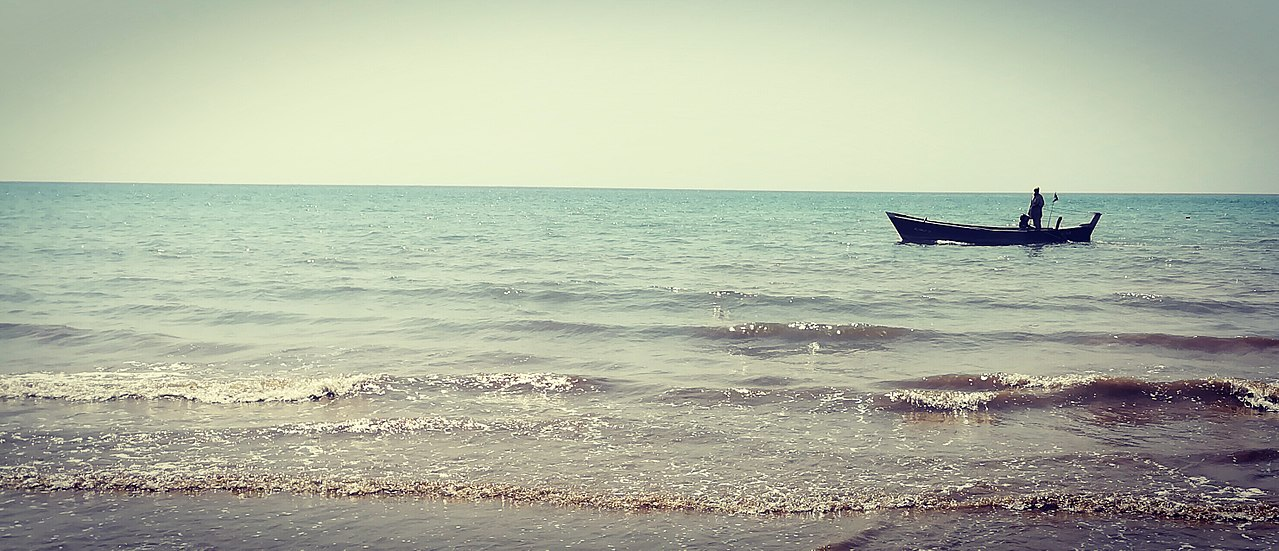
\includegraphics{seaside}
	\caption[A wide seaside]{A wide seaside, and a wide caption.
		Credits: By Bushra Feroz, CC BY-SA 4.0, \url{https://commons.wikimedia.org/w/index.php?curid=68724647}}
\end{figure*}

\begin{marginfigure}
	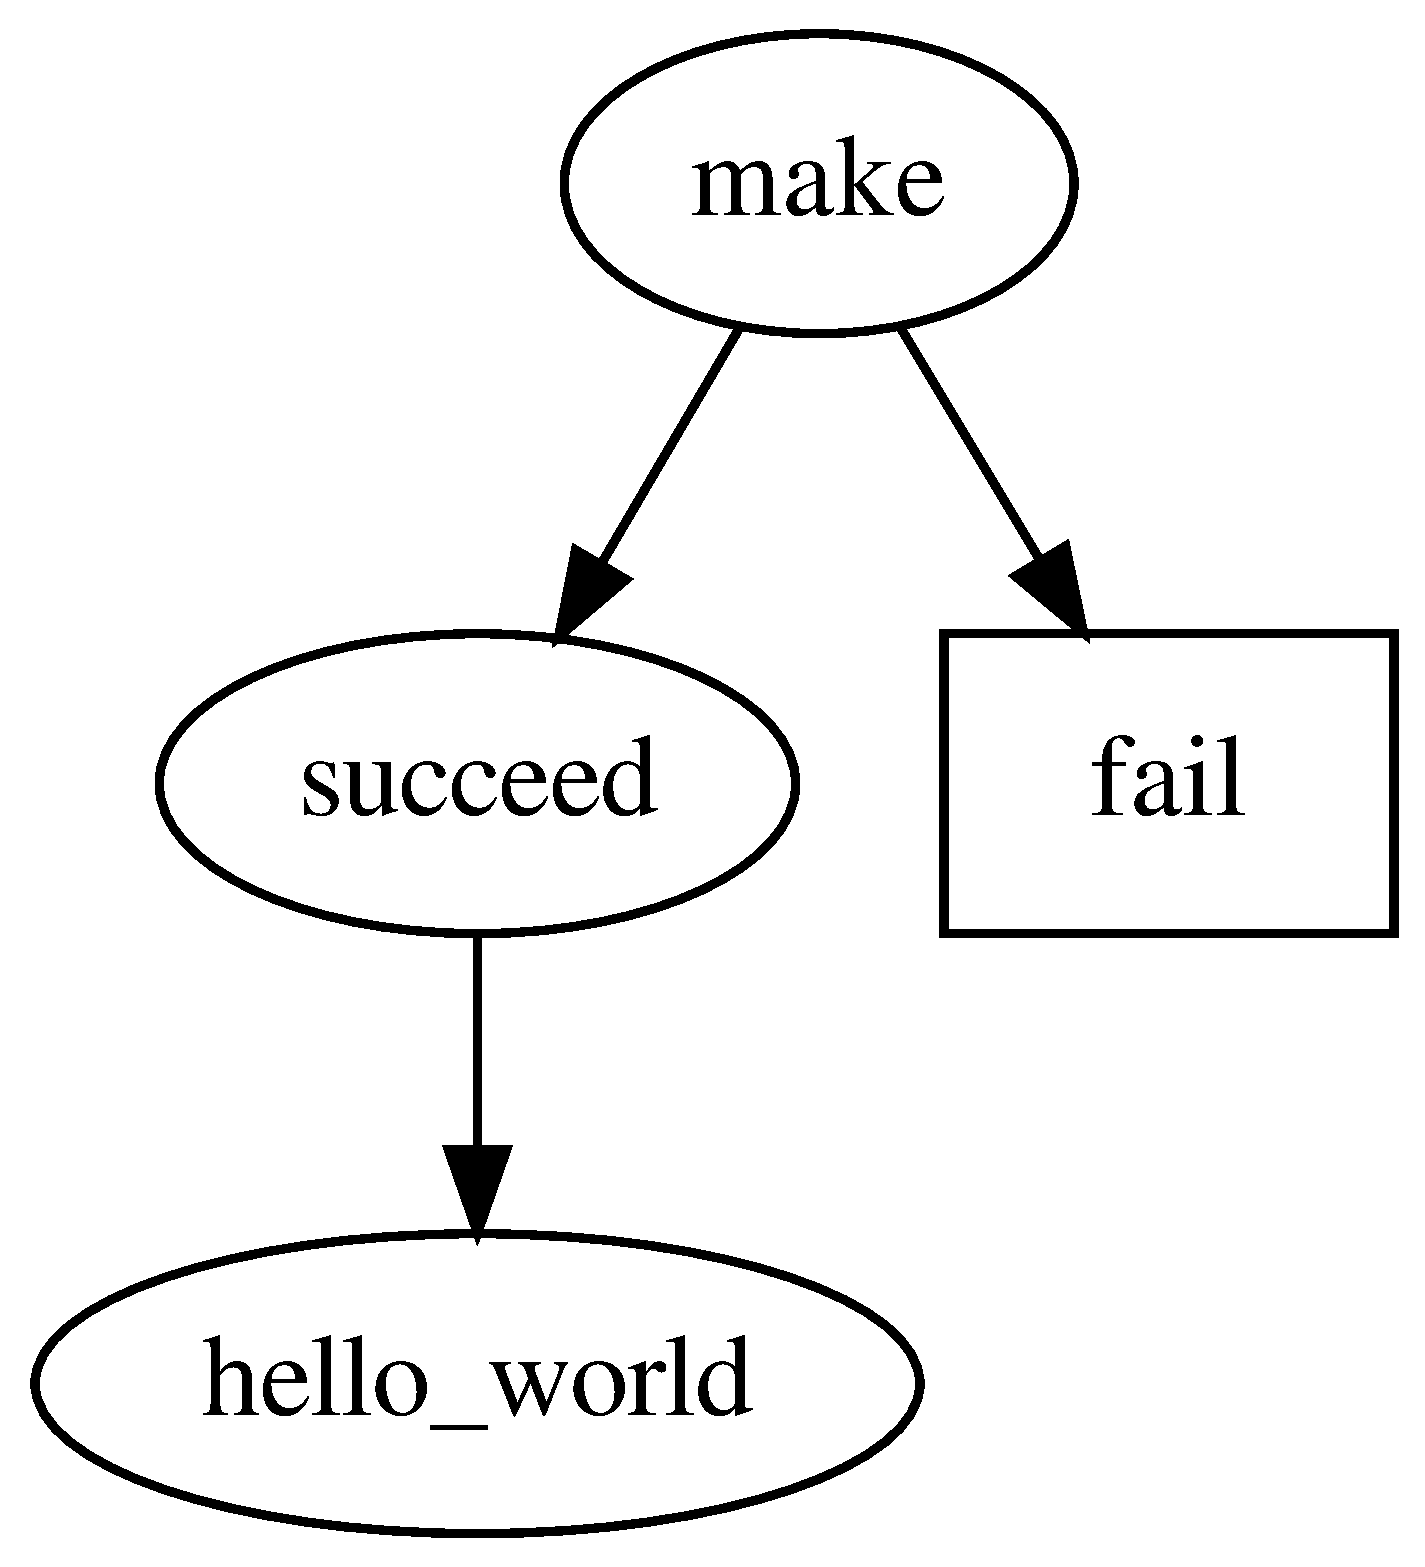
\includegraphics{output2}
	\caption[A Dot diagram]{A diagram produced by the Dot program and saved as a PNG file.}
	\labfig{marginmonalisa}
\end{marginfigure}


%
% Subsection: Citations
%------------------------------------------------------------------------------
\subsection{Citations}
Cite an author in the margin\sidecite{example1999}.

\blindtext


%
% Subsection: Glossaries and Indicies
%------------------------------------------------------------------------------
\subsection{Glossaries and Indicies}

%
% Subsection: Mathematics
%------------------------------------------------------------------------------
\subsection{Mathematics}
The box below was created using the \Environment{definition} environment. Boxes are also
provided by the \Environment{theorem}, \Environment{proposition}, \Environment{lemma},
\Environment{corollary}, \Environment{example}, \Environment{remark}, and \Environment{exercise} environments.

\begin{definition}
\labdef{exdeflabel}
Let $y$ be some function of $x$ such that $y = f(x)$
\end{definition}

where $x$ and $y$ are both variables in \refdef{exdeflabel}.



\blindtext

%
% Chapter Review
%==============================================================================
\section{Chapter Review}
\begin{kaobox}[frametitle=Chapter Review]
you have learned
\begin{itemize}
	\item what is the first topic
	\item how to identify the second topic
        \item best practices for the third topic
\end{itemize}

you are able to
\begin{itemize}
        \item perform the steps required to accomplish task one
        \item create a program that performs task two
\end{itemize}
\end{kaobox}






